\chapter{IoT \& Backscattering}
In this chapter we begin with the Internet of Things — what it really means, what “things” are, and why this topic matters now. 
Then we move to a focused and increasingly practical question: can smart objects work without batteries? The answer opens a fascinating area: battery-free IoT and backscattering techniques.

\section{What is the Internet of Things (IoT)?}
When people say “\textit{Internet of Things}” they usually mean one or more of three related things. 
\begin{itemize}
    \item First, it can mean the global network formed when everyday objects become able to sense, compute, and communicate — not just phones and laptops, but tiny devices embedded in the physical world. 
    \item Second, IoT refers to the collection of technologies that make that interconnection possible: addressing and naming schemes, wireless access technologies, low-power electronics, data formats and management systems, and so on. 
    \item Third, IoT describes the set of applications and services that run on top of those networks and technologies — for example, smart home energy management, fleet tracking, or automated inventory in a warehouse.
\end{itemize}
Think of IoT as both an infrastructure idea (lots of tiny devices connected) and an ecosystem (technology stacks plus services and business models built on top).

When we ask “what kind of things,” the straightforward answer is: everything that becomes “smart.” A smart object is an ordinary physical thing that has electronics embedded so it can compute and exchange information. Common examples are obvious: smartwatches, phones, TVs. But the IoT idea reaches far beyond consumer gadgets. When cars, buildings, streetlights, or entire city systems can sense and communicate, they become part of the IoT.

A helpful way to think about IoT is to ask whether a smart object can do three things.
\begin{enumerate}
    \item It must be \textit{identifiable}. If anything in the environment can be addressed, discovered, and tied to an identity, then systems and services can reason about it.
    \item It has to \textit{communicate}. That means at least minimal networking capabilities — the ability to receive messages or commands and to send responses.
    \item Third, it must \textit{interact}. Interaction can be between devices — building ad hoc, local networks — or between a device and a human.
\end{enumerate}
A single smart object usually combines five basic aspects.
\begin{enumerate}
    \item It has a physical body: size, shape, casing, connectors, and placement matter a lot because they affect the environment the device senses and how it communicates.
    \item It offers basic communication functionality: discovery, accepting messages, and replying.
    \item It has at least one name and one address so that other entities can refer to it and route messages to it.
    \item It has some compute ability; even very limited processors can match incoming messages to fingerprints, apply simple filters, or run control logic.
    \item It has means to observe the physical world (sensors for temperature, light, motion) or to act on it (actuators that turn a relay on, move a motor, or switch a valve). That sensing/acting capability is what differentiates smart objects from routers or servers in the classical Internet.
\end{enumerate}
Many devices in IoT come from two well-established areas: RFID and wireless sensor networks (WSNs). RFID focuses on identification and very low-power tags, while WSNs focus on distributed sensing and multi-hop communication. IoT includes both but also devices that may have only the most basic communication and compute stacks — sometimes not a full TCP/IP stack. The unifying view of IoT is about objects acting as providers or consumers of data that describe the physical world.

Putting millions — or billions — of small, smart objects into the world creates a long list of system requirements. Let me walk you through the most important ones.
\begin{itemize}
    \item \textit{Devices heterogeneity:} devices differ widely in CPU power, memory, radio capabilities, and energy sources. The network and protocols must accommodate that diversity gracefully.
    \item \textit{Scalability:} naming, addressing, routing, data management and service discovery must scale to huge numbers of devices distributed over large physical areas.
    \item \textit{Ubiquitous local data exchange:} many use cases need local wireless proximity networking (for example, a smart meter talking to a gateway), and that requires efficient use of radio spectrum and reliable short-range communication.
    \item \textit{Energy optimization:} many devices run on small batteries or on harvested energy. Energy is often the most scarce resource, motivating careful duty cycling, low-power radios, and sometimes entirely battery-free designs.
    \item \textit{Localization and tracking:} numerous applications require knowing where a device is — asset tracking, logistics, and animal tagging among them — so position estimation and tracking methods are necessary.
    \item \textit{Self-organization:} devices may come and go, so networks must form ad hoc, adapt to topology changes, and recover from partitions with minimal central control.
    \item \textit{Semantic interoperability and data management:} the data coming from millions of heterogeneous sensors must be interpretable. That means common formats, metadata, and possibly ontologies to make data shareable and meaningful across applications.
    \item \textit{Security and privacy:} without strong, built-in mechanisms for authentication, confidentiality, and data protection, users and organizations won’t accept IoT systems.
\end{itemize}
To turn the conceptual pillars into reality, devices need a set of enabling capabilities: identification, communication, computation, and direct interaction with the physical environment. Two of the key building technology families for these are wireless sensor networks and RFID. WSNs bring networking theory, routing, and energy-aware MAC protocols; RFID contributes ultra-low-power identification and the idea of passive tags. 

\section{Battery-free smart objects}
Can we redesign smart objects so they work without batteries? The answer is yes — at least for a class of low-power devices — and the enabling trick is called backscattering.

\textit{Backscattering} is a simple physical idea: instead of generating a radio signal actively, a device modifies how much of an incoming radio wave it reflects (see Figure \ref{fig:backscattering}). By toggling that reflection in controlled ways, the device encodes information into the reflected wave. Since the device does not need to create its own RF carrier, the energy cost can be orders of magnitude lower.

\begin{figure}[ht]
    \centering
    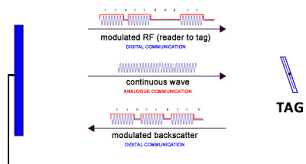
\includegraphics[width=0.7\linewidth]{images/backscattering.png}
    \caption{Backscattering.}
    \label{fig:backscattering}
\end{figure}

Backscatter systems can sometimes harvest the energy they need from the illuminating radio waves themselves, which eliminates the need for an on-board battery. That’s why they’re often called battery-free or passive devices.

Consider a radio reader or a Wi-Fi transmitter shining electromagnetic energy across a space. A passive tag sits in that field and uses an antenna and a tiny rectifier to pull out a little bit of energy. The tag doesn’t amplify and transmit; it instead changes its antenna impedance to reflect more or less of the incoming wave. That controlled change in reflection appears as variations in the signal the reader receives. The reader senses those variations and demodulates the data the tag encoded.

Two common backscattering flavors are \textit{ambient backscatter} and \textit{RFID backscatter}.
\begin{itemize}
    \item Ambient backscatter devices don’t rely on a dedicated reader. Instead, they harvest energy from existing RF transmissions in the environment — TV broadcasts, cellular towers, or nearby Wi-Fi access points. Since those signals are already present, an ambient backscatter tag can reflect them to send information without requiring any new infrastructure.

    Ambient backscattering tends to have very low data rates, typically below 1 kilobit per second. This makes it suitable for applications that only need to send tiny bursts of information occasionally — for instance, a passive sensor that reports whether an item is present or not. It’s not suitable for real-time streaming or frequent updates.

    Another limitation is signal availability. Even though some signals (like TV towers) broadcast continuously, you can’t assume uniform coverage everywhere. In practice, signals can be weak indoors and may drop off sharply with distance or be blocked by buildings. If the ambient signal is too weak, the device can’t harvest enough energy to power even its minimal electronics.
    
    \item In RFID systems the reader is part of the design. The reader emits a continuous RF signal (the carrier), and passive RFID tags harvest energy from that signal to run a tiny circuit. To communicate, the tag modulates the reflection of the reader’s signal. Because the reader is present and controllable, RFID systems typically have better performance and predictable availability compared to ambient backscatter.

    This predictability is the main advantage: when a reader is present, it supplies both the energy and the receiver that decodes the tag’s reflection. That enables longer ranges, better data reliability, and higher effective throughput in many deployments.
\end{itemize}
RFID systems are heavily used in logistics, retail, and access control because of this dependable reader-tag model.
RFID tags originally were used primarily for identification: a tiny ID number the reader interrogated. But the technology scales: you can add sensors to tags so they measure motion (accelerometers), occupancy or motion (PIR sensors), or even small cameras in very constrained setups. These are called sensor-augmented RFID tags.

The idea is powerful: combine passive energy harvesting with embedded sensing so a tag can both say “I am item X” and also report a sensed value like temperature or whether a package has been opened. Because the tag can harvest energy from the reader, it can sometimes power these sensors for short periods.

However, these tags face fairly strict constraints. They have limited power because they only harvest what the reader transmits and what the antenna/rectifier can capture. Their operating range is short compared to active radios — the reader typically has to be close. The time they can operate continuously is limited (they may need to accumulate charge between transmissions), and their available storage is small so they can’t buffer much data. Data rates tend to be low compared with smartphones or Wi-Fi devices. Yet, despite these limits, they can run small sensors and provide valuable sensing data at very low cost and with near-zero maintenance (no battery to replace).

The research group built real, playable devices to prove the concept.
One example is \textit{SapyJoy}, a battery-free video game controller. The team mounted an analog joystick and two buttons onto a Moo tag and wired them through a small PCB. Because the Moo tag also contains an accelerometer, the controller supports richer, complex inputs. When the reader energizes the tag, the tag harvests power and quickly encodes joystick positions and button presses into backscattered payloads that the server translates into game inputs. Because the microcontroller on the tag can measure the analog joystick and encode that into the tag’s payload, the controller can be used for real games though responsiveness depends on how frequently the reader polls tags and how many other devices share the channel.

A similar idea maps to a battery-free mouse: the x and y axes are read by the tag and translated into pointer motion on the host. This requires precise timing and small latencies so the cursor movement feels smooth.

The group also built a battery-free light switch by mounting a button onto a Moo tag. Pressing the tag button triggers an event when the reader energizes the tag; the server receives the sensor payload and toggles the target LED or light fixture. Multiple buttons can be exposed on a single tag to control different lights; the logical mapping between the tag and the actuator is implemented in the server so the tag remains simple.

These demos show that almost every small human interface can be reimagined as a passive RFID device, but they also expose scalability and timing limitations.

The tags in this work use \textit{EPC Gen2} — the ubiquitous standard for passive UHF RFID — but with a twist. The standard defines memory banks primarily for storing tag IDs. In practical deployments a full ID field (commonly 96 bits) isn’t always necessary, so researchers repurpose spare bits.

The particular experiment limited the data field such that one byte is reserved for a compact tag identifier while six bytes are used for sensor data (this payload includes the CRC bits used for error checking — in the team’s case, four bits of CRC are included in the payload accounting). The reason for keeping the payload short is robustness: shorter payloads decrease packet error rates under the weak-signal, noisy conditions typical of backscatter links. The only device that would require more payload than this architecture supports is a camera; even small image data would have to be fragmented into many backscatter frames.

A few practical details worth understanding. The tiny tag still needs to compute a CRC (cyclic redundancy check) for its payload to help the reader detect bit errors in reception; CRC computations can be implemented in small, energy-efficient logic. Because backscatter links have constrained throughput and intermittent availability, the entire cycle of harvest → sense → compute → modulate → sleep must be designed to fit the tag’s energy budget and the application’s latency requirements.

In the experiments the team used a USRP (a software-defined radio) as the RFID reader. A USRP allows flexible control of the carrier and reception chain.

Two antenna ports per room (one for Tx and one for Rx) let the reader separate the forward carrier from the weak backscattered signal. On the signal-processing side, a matched filter was used in the SapyJoy demo. A matched filter is a classic detector that maximizes signal-to-noise ratio (SNR) when you know the waveform you expect; by correlating the incoming signal with the known pattern (or expected symbol shape), the receiver becomes more resilient to noise. In practice, matched filtering means the reader can better decode the tiny, reflected modulations coming from the tag and so reduce packet errors or improve range.

For interactive and environmental applications the reaction time is the key metric. Reaction time is defined as the time interval between the generation of a new sensor reading and the time an application reacts to it. For the joystick, reaction time measures the time from when the user moves or presses a control to when the game reacts. For a presence sensor connected to a camera, reaction time measures the time between the physical event (someone entering a room) and a camera starting to record or an alarm being raised.

Testing one device at a time hides the biggest challenge: simultaneous operation. When multiple passive devices share a reader, they must be polled, scheduled, or otherwise coordinated to avoid collisions and to make sure each tag can harvest enough energy to operate.

The experiments used a time-division multiple access (TDMA) style approach: the reader cycles through timeslots, polling different tags in a repetitive frame. If a device is polled every slot, it gets low reaction time; if it is polled once every many slots, its reaction time increases. In a three-device experiment (two environmental sensors and the joystick) the reaction time for the joystick increased from about 93 ms when alone to about 200 ms when sharing the channel. That doubling shows the impact of multiplexing: more devices implies longer wait times between opportunities to harvest and transmit.

With more devices (40 devices in simulation), naive equal allocation leads to unacceptable delays for interactive devices. That’s where smarter MAC strategies are required.

The research identifies a clear open problem: equal allocation of channel resources doesn’t satisfy the widely varying needs of heterogeneous devices. A joystick demands low latency under high activity, while a temperature sensor is content with sporadic updates. Static slotting is inefficient and leads to long delays for interactive devices as the number of devices grows.

Adaptive protocols like APT-MAC show a path forward, but the general problem remains: what is the best tradeoff between fairness, responsiveness, and energy distribution when devices cannot generate their own energy and must wait for reader energization? This question touches MAC design, power control, scheduler fairness, application priorities and even economic or user policy choices (who gets priority: safety sensors or entertainment devices?).

Imagine you could draw a button on a napkin, stick a tiny sticker-sized RFID chip on it, and turn that doodle into a real wireless input. \textit{JoyPaper} does exactly that: it uses commercially available ultra-compact UHF RFID integrated circuits in sticker form, conductive-ink pens, and plain paper to make interactive, battery-free tags you can draw by hand (see Figure \ref{fig:joy-paper}).

The basic materials are simple. You start with a small loop IC packaged as a sticker; these are the off-the-shelf RFID chips that normally sit on labels. Then you draw conductive traces on paper using a pen filled with conductive ink. The sticker is placed over the traces so that when the printed antenna path is complete, the loop IC has a functioning antenna and behaves like a normal passive RFID tag.

\begin{figure}
    \centering
    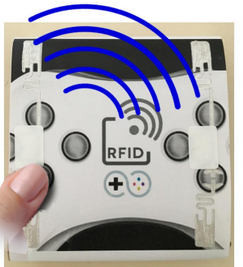
\includegraphics[width=0.4\linewidth]{images/joy-paper.png}
    \caption{JoyPaper.}
    \label{fig:joy-paper}
\end{figure}

What’s clever about JoyPaper is that the conductive traces can be designed so that touching or pressing a particular spot restores antenna continuity. That touch turns the tag into an input sensor. In other words, the act of pressing a paper button physically closes (or opens) a conductive path which switches the tag from “silent” to “active.” When the tag is active and a reader is querying the environment, it harvests power from the reader’s carrier and sends its ID. The reader — or a server attached to it — then interprets that ID as a button press or other input event.

\section{Infrastructure-based wireless networks}
This is the model you use every time when your phone connects to a cell tower (see Figure \ref{fig:infrastructure-based-wn}). You have base stations (GSM, UMTS, LTE, 5G) or Wi-Fi access points that are connected to a wired backbone. Mobile devices speak to base stations; the base stations forward traffic over the wired network; handovers let users move from one base station to another while maintaining connections. Routers, gateways and servers in the backbone carry and manage traffic, authentication, billing, and other administrative tasks.

\begin{figure}[ht]
    \centering
    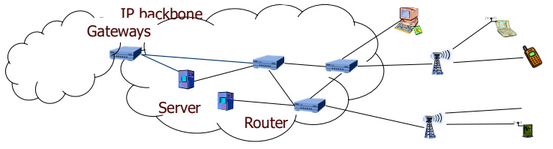
\includegraphics[width=0.7\linewidth]{images/infrastructure-based-wn.png}
    \caption{Infrastructure-based Wireless Networks.}
    \label{fig:infrastructure-based-wn}
\end{figure}

There are many situations where the necessary infrastructure is missing or impractical. Maybe you’re in a disaster zone where the towers and wired links are down. Maybe you’re on a remote construction site or in a rural area where no operator provides coverage. Sometimes deployment time is tight — in military or emergency operations you can’t wait to build a fixed network. Even a house or a temporary event might not be connected to a backbone in the way you want.
Those scenarios motivate infrastructure-less networking.

\section{Infrastructure-less networks and MANETs}
If you can’t rely on base stations or backbone routers, you build networks with the devices you have. That’s the idea behind ad hoc networks and, in particular, \textit{Mobile Ad Hoc Networks (MANETs)}. In a MANET each node — whether it’s a laptop, a phone, a vehicle or an embedded device — participates in building the network. Nodes forward packets for others, discover neighbors, and coordinate access to the shared wireless medium all without a central controller.

Picture a set of laptops in a conference room sharing slides directly with each other—no Wi-Fi access point necessary. Or imagine first responders at a disaster site all wearing devices that must communicate even though the usual infrastructure is offline. Car-to-car communication for cooperative driving is another natural fit: vehicles exchange information directly about speed or hazards. A search-and-rescue team in an avalanche can use an ad hoc network to find victims and coordinate routes without relying on a distant server. Even everyday services — finding empty parking spaces by local broadcast, or a soldier platoon coordinating movement — can be enabled by MANETs. Smaller scale personal area networks (smartwatch, glasses, medical sensors) are another form of infrastructureless networking, often with tight energy and latency constraints.

Building a functioning ad hoc network requires solving a cluster of problems that are mostly hidden by infrastructure in cellular or Wi-Fi networks. The main challenges are the absence of a central organizing entity, limited radio range, node mobility, and constrained energy supplies.

Nodes have to discover each other, decide who should transmit when, and figure out paths to forward traffic. All of that happens in a distributed, self-organizing way. There’s no base station to assign resources or to route packets, so protocols must do neighbor discovery, medium access control (MAC), and routing cooperatively.

MAC in infrastructure networks is often simple because the base station can schedule or coordinate transmissions. In ad hoc networks everyone shares the medium. The MAC must therefore solve classic distributed problems like avoiding collisions, dealing with the hidden terminal problem, and allowing fair or prioritized access. Common approaches include CSMA/CA (listen before talk), distributed TDMA variants, or hybrid approaches, but each has tradeoffs in overhead, energy use, and fairness.

Because radio range is short and obstacles can block signals, direct communication to a distant node is often impossible. The solution is multi-hop routing: nodes forward packets through intermediate neighbors. But routing without infrastructure is tricky. As nodes move, routes break and must be discovered or repaired. This requires constant or on-demand control traffic, which consumes bandwidth and energy. Scalability is also an issue: route maintenance becomes more burdensome as networks grow.

Mobility changes the neighborhood graph continuously, so routes and local state must be updated fast enough to remain useful. Some routing schemes proactively maintain routes, costing continuous overhead, while others discover routes on demand, which introduces delay when a path is first needed. Balancing responsiveness and control overhead is central to MANET protocol design.

Multi-hop routing can sometimes save energy because transmitting over many short hops can be cheaper (in energy per bit) than a single long transmission that requires many more watts. But that’s not always true: relaying packets costs energy for the forwarder, and nodes that forward a lot may die early, hurting overall network lifetime. Designing energy-aware routing means balancing per-link energy costs, fairness, and the network’s longevity.

Multi-hop networks also complicate latency and reliability. Each hop introduces delay and a chance of packet loss, so protocols must mitigate errors (retransmissions, forward error correction) and manage queuing at intermediate nodes.

Most devices in ad hoc networks are battery powered. For many applications, maximizing the lifetime of an individual device and the network as a whole is a primary design goal. That leads to energy-efficient strategies: duty cycling radios so they sleep most of the time, choosing routes that minimize energy per delivered bit, using wake-on-event sensors, or employing cooperative techniques where nodes alternate forwarding responsibilities to avoid draining any single node.

But energy optimization is a multi-objective problem. You might optimize for latency, or reliability, or fairness, and those goals often conflict with minimizing energy consumption. Designers must choose what to prioritize: for example, in a life-saving application you accept higher energy use for lower latency; in a long-term environmental monitoring deployment you favor energy savings at the cost of higher delay.

Despite intense research into ad hoc networking for decades, a single, mass market “killer app” that requires pure infrastructureless, large-scale MANETs has been elusive. Many specialized applications succeeded or found niches, like tactical military networks or sensor networks, but the broad consumer market adopted infrastructureed solutions because they are easier to monetize and control.

Sensor networks — a close relative of ad hoc networks — achieved greater practical success because their topology and traffic patterns are usually more predictable, they focus on energy efficiency and multi-hop strategies optimized for many low-rate sensors, and the application domains (environmental monitoring, industrial sensing) map well to their constraints.